
\documentclass{beamer}

\usepackage{algpseudocode, color, colortbl}

\usepackage{sudoku}
\setlength\sudokusize{3cm}
\renewcommand*\sudokuformat[1]{\tiny#1}

\usepackage{hyperref}
\hypersetup{
    colorlinks=true,
    urlcolor=blue,
}

\usetheme{Montpellier}
\usecolortheme{rose}

% page numbers, from
% https://tex.stackexchange.com/questions/137022/how-to-insert-page-number-in-beamer-navigation-symbols
\expandafter\def\expandafter\insertshorttitle\expandafter{%
  \insertshorttitle\hfill%
  \insertframenumber\,/\,\inserttotalframenumber}

\definecolor{Gray}{gray}{0.8}
\newcolumntype{g}{>{\columncolor{Gray}}c}

\newcommand{\stanza}{ \\~\ }

\title{10. Integer Linear Programming}
\subtitle{CPSC 535}
\author{Kevin A. Wortman}
\institute{ 
\includegraphics[height=2cm]{csuf-logo-cmyk} }
\date{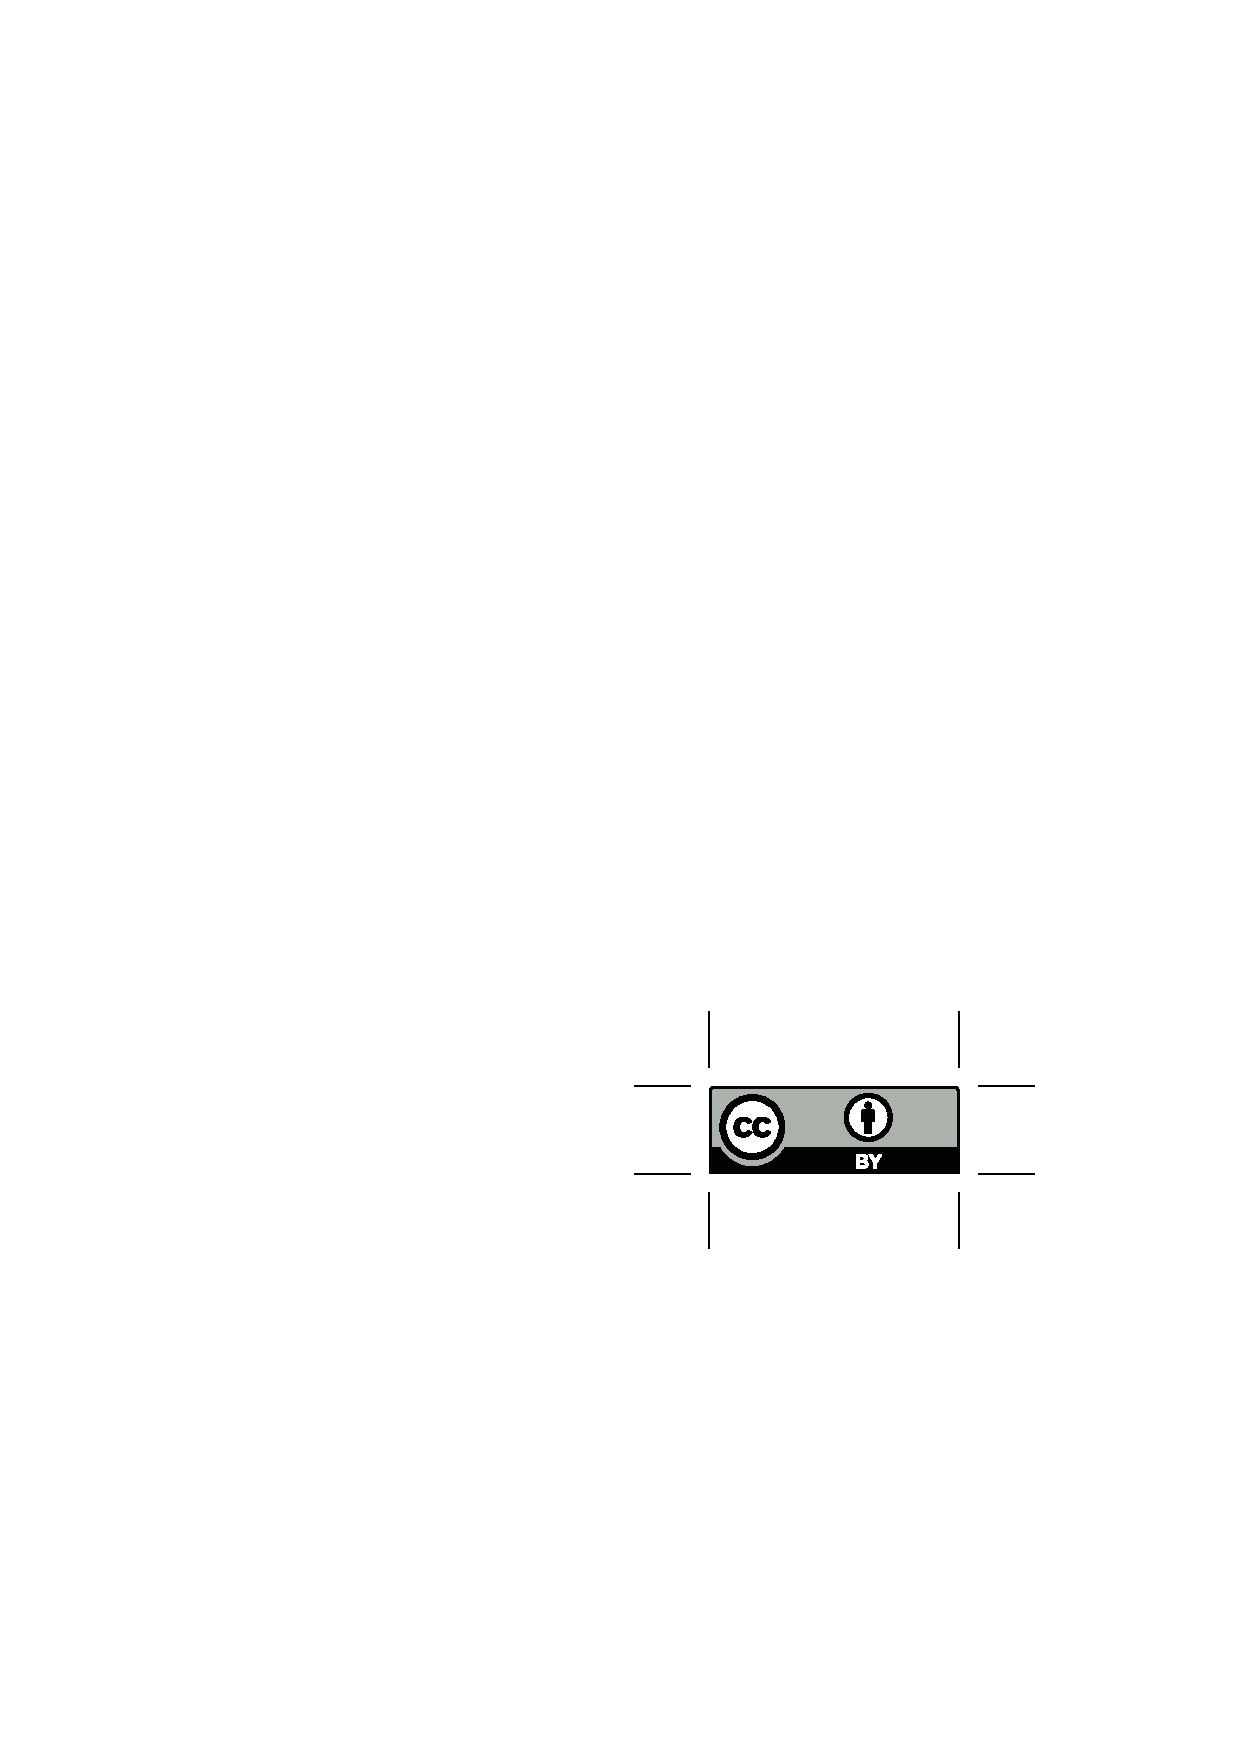
\includegraphics[height=14pt]{by} \\

{\tiny
This work is licensed under a
\href{http://creativecommons.org/licenses/by/4.0/}{Creative Commons Attribution 4.0 International License}.
}}

\begin{document}

\begin{frame}
  \titlepage
\end{frame}

\begin{frame} \frametitle{Recall: General LP Problem}
  \emph{general-form linear programming problem} \\
  \textbf{input:}
  \begin{itemize}
    \item Boolean for whether $f$ is maximized/minimized
    \item vector $c \in \mathbb{R}^n$
    \item vector $b \in \mathbb{R}^m$
    \item vector $o \in \{\leq, =, \geq\}^m$
    \item $m \times n$ matrix $A$ of real numbers
  \end{itemize}
  \textbf{output:} one of
  \begin{enumerate}
    \item ``unbounded'';
    \item ``infeasible''; or
    \item ``solution'' with a vector $x \in \mathbb{R}^n$
      maximizing the objective function
  \end{enumerate}
\end{frame}

\begin{frame} \frametitle{Recall: Reduction Algorithm}

  {\footnotesize
  \begin{algorithmic}[1]
    \Function{SOLVE-A}{input-for-A}
    \State input-for-B = pre-process input-for-A
    \State solution-for-B = solve-B(input-for-B)
    \State solution-for-A = post-process solution-for-B
    \State \Return{ solution-for-A }
    \EndFunction
  \end{algorithmic}
  }

\end{frame}

\begin{frame} \frametitle{Algorithms that Reduce to LP}

  {\footnotesize
  \begin{algorithmic}[1]
    \Function{SOLVE-A}{input-for-A}
    \State program = convert input-for-A to linear program
    \State result = solve-B(input-for-B)
    \If{ result is "unbounded"}
      \State return output-for-unbounded-case
    \ElsIf{ result is "infeasible"}
      \State return output-for-infeasible-case
    \Else
      \State solution-for-A = convert LP solution
      \State \Return{ solution-for-A }
    \EndIf
    \EndFunction
  \end{algorithmic}
  }

\end{frame}

\begin{frame} \frametitle{Integer Linear Programming}
  \begin{itemize}
  \item \emph{\textbf{integer} linear programming:} like general form, but all variables are integers instead of real
  \item i.e. each $x_i \in \mathbb{Z}$
  \item \emph{Mixed Integer Programming (MIP):} mixture of real and integer variables
  \item i.e. a subset $I \subseteq \{x_1, \ldots, x_n\}$ of variables are restricted to integers
  \end{itemize}
\end{frame}

\begin{frame} \frametitle{MIP problem}
  \emph{mixed-integer programming problem (MIP)} \\
  \textbf{input:}
  \begin{itemize}
    \item Boolean for whether $f$ is maximized/minimized
    \item vector $c \in \mathbb{R}^n$
    \item vector $b \in \mathbb{R}^m$
    \item vector $o \in \{\leq, =, \geq\}^m$
    \item $m \times n$ matrix $A$ of real numbers
    \item set $I \subset \{1, \ldots, n\}$
  \end{itemize}
  \textbf{output:} one of
  \begin{enumerate}
    \item ``unbounded'';
    \item ``infeasible''; or
    \item ``solution'' with a vector $x \in \mathbb{R}^n$
      maximizing the objective function; if $i \in I$ then $x_i \in \mathbb{Z}$
  \end{enumerate}
\end{frame}

\begin{frame} \frametitle{MIP Applications}
  \begin{itemize}
  \item \textbf{discrete variables:} can formulate a business-logic whole number concept with
  \begin{itemize}
    \item variable $x_i, i \in I$
    \item example: you can buy 3 or 4 airplanes but not 3.7
  \end{itemize}
  \item \textbf{true/false decision:} can formulate a true/false choice with
    \begin{itemize}
    \item variable $x_i$, $i \in I$
    \item constraints $0 \leq x_i$ and $x_i \leq 1$
    \end{itemize}
\item \textbf{choose among $k$ alternatives:} more generally, can
  formulate a choice from $\{a, \ldots, b\} \subset \mathbb{Z}$ with
  \begin{itemize}
  \item variable $x_i, i \in I$
  \item constraints $a \leq x_i$ and $x_i \leq b$
    \end{itemize}
  \end{itemize}
\end{frame}

\begin{frame} \frametitle{MIP Hardness}
  \begin{itemize}
  \item Recall: hardness of general LP is an open question
  \item not proven in $P$, not proven $NP$-hard
  \item MIP \textbf{is} $NP$-complete
  \item specifying integer variables seems to make the problem substantially harder
  \item worst-case MIP programs are intractible
  \item \textbf{but} MIP solvers use lots of clever heuristics
  \item so specific MIP formulations are often computationally feasible in practice
  \end{itemize}
\end{frame}

\begin{frame} \frametitle{Vertex Cover}
  \emph{vertex cover problem} \\
  \textbf{input:} an undirected graph $G=(V, E)$ \\
  \textbf{output:} a vertex cover $C$ of minimum size
  \stanza

  \emph{vertex cover:} a subset $C \subseteq V$ such that, if $(u, v) \in E,$ then $u \in C$ or $v \in C$ (or both)
 
  \begin{center}
    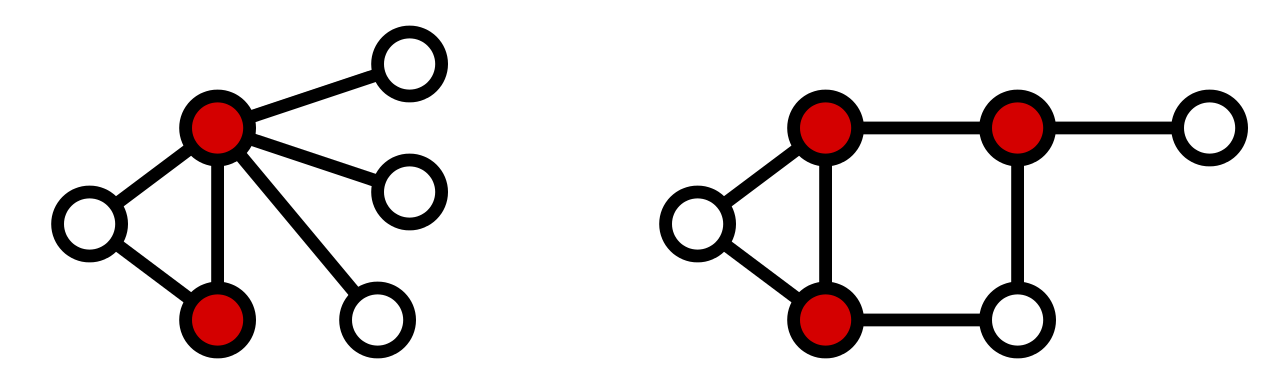
\includegraphics[height=1in]{vertex-cover.png} \\
    {\tiny Image credit: \url{https://commons.wikimedia.org/wiki/File:Minimum-vertex-cover.svg} }
  \end{center}

\end{frame}

\begin{frame} \frametitle{Formulating Vertex Cover}
  \textbf{Recall:}
  \begin{itemize}
    \item vertex cover is $NP$-complete
    \item if vertex cover can be formulated as a MIP problem, then MIP is $NP$-hard
    \stanza
  \end{itemize}

  ``Rules'' to represent:
    \begin{itemize}
      \item each vertex is either in $C$ or not
      \item each edge has at least one end in $C$
      \item minimize $|C|$
    \end{itemize}
\end{frame}

\begin{frame} \frametitle{Formulating Vertex Cover}
\textbf{Variables:} for each $v \in V$, create an integer variable $x_v$ such that
\[ x_v = 1 \Leftrightarrow v \in C \]

\textbf{Objective:} minimize
\[ \sum_{v \in V} x_v \]

\textbf{Constraints:}
\begin{tabular}{lll}
  $0 \leq x_v \leq 1$ & $\forall v \in V$ & (0 or 1 indicator) \\
  $x_u + x_v \geq 1$ & $\forall (u, v) \in E$ & (each edge is covered)
\end{tabular}

\end{frame}

\begin{frame} \frametitle{Vertex Cover Outcomes}
  \begin{itemize}
    \item \textbf{Infeasible:}
      \begin{itemize}
      \item never happens
      \item $\exists$ a solution: setting all $x_v=1$ satisfies all constraints
      \end{itemize}
    \item \textbf{Unbounded:}
    \begin{itemize}
      \item never happens
      \item objective is bounded: the objective function is to minimize 
        \[ \sum_{v \in V} x_v; \]
        since every $x_v \geq 0$, the minimum objective value is zero, which is finite, so the program is never unbounded
    \end{itemize}
    \item \textbf{Solution:} Construct $C$ as
      \[ C = \{ v \,|\, v \in V \text{ and } x_v=1 \} \]
    \end{itemize}
  \end{frame}

  \begin{frame} \frametitle{TSP}
    \emph{traveling salesperson problem (TSP)} \\
    \textbf{input:} a complete, weighted, undirected graph $G=(V, E)$ \\
    \textbf{output:} a tour $T$ of minimum weight
    \stanza

    \emph{tour:} a sequence of vertices $\langle t_1, \ldots, t_n \rangle$
    that visits each vertex exactly once \emph{Hamiltonian cycle}
    \stanza
  
    Define: \\
    \[ n \equiv |V| \]
    \[ w(u, v) \equiv \text{ the weight of the edge from } u \text{ to } v \]
  \end{frame}
  
  \begin{frame} \frametitle{Formulating TSP}
    ``Rules'' to represent:
      \begin{itemize}
        \item each vertex is visited exactly once
        \item minimize total weight
      \end{itemize}
  \end{frame}
  
  \begin{frame} \frametitle{Formulating TSP}
  \textbf{Variables:} for each $u \in V$ and $v \in V,$ create an integer variable $x_{u, v}$ such that
  \[ x_{u,v} = 1 \Leftrightarrow \text{ the tour steps from } u \text{ to } v \]
  
  \textbf{Objective:} minimize
  \[ \sum_{u, v \in V} w(u, v) \cdot x_{u, v} \]
  
  \textbf{Constraints:}
  \begin{tabular}{lll}
    $0 \leq x_{u, v} \leq 1$ & $\forall u, v \in V$ & (0 or 1 indicator) \\
    $\sum_{u \in V} x_{u, v} = 1 $ & $\forall v \in V$ & (each vertex is entered once) \\
    $\sum_{v \in V} x_{u, v} = 1 $ & $\forall u \in V$ & (each vertex is exited once) \\
    $\sum_{u, v \in V} x_{u, v} = n$ & & (tour has $n$ edges) 
  \end{tabular}
  
  \end{frame}
  
  \begin{frame} \frametitle{TSP Outcomes}
    \begin{itemize}
      \item \textbf{Infeasible:}
        \begin{itemize}
        \item never happens
        \item $\exists$ a solution: $G$ is complete, so certainly contains at least one tour
        \end{itemize}
      \item \textbf{Unbounded:}
      \begin{itemize}
        \item never happens
        \item objective is bounded: observe that $\sum_{u, v \in V} w(u, v) \cdot x_{u, v}$
          is minimized when every $x_{u,v}$ is zero; so the minimum objective value is zero; which is finite.
      \end{itemize}
      \item \textbf{Solution:} Construct $T=\langle t_1, \ldots, t_n \rangle$ as
       \[
        t_i =
        \begin{cases}
          \text{an arbitrary } v \in V & i=1 \\
          v \text{ such that } x_{t_{i-1}, v}=1 & i>1 
        \end{cases}
       \]
      \end{itemize}
    \end{frame}
  
\begin{frame} \frametitle{Formulating Sudoku}
  \textbf{Sudoku:} input is a $9 x 9$ grid, some cells are integers $\{1, \ldots, 9\},$ others are blank

  \begin{sudoku}
    | | | |2|6| |7| |1|.
    |6|8| | |7| | |9| |.
    |1|9| | | |4|5| | |.
    |8|2| |1| | | |4| |.
    | | |4|6| |2|9| | |.
    | |5| | | |3| |2|8|.
    | | |9|3| | | |7|4|.
    | |4| | |5| | |3|6|.
    |7| |3| |1|8| | | |.
  \end{sudoku}
  
  Rules:
  \begin{enumerate}
  \item Objective: fill every blank
  \item Each row contains $\{1, \ldots, 9\}$
  \item Each column contains $\{1, \ldots, 9\}$
  \item Each $3 \times 3$ subgrid contains $\{1, \ldots, 9\}$
  \item (implies none of these regions has duplicates)
  \end{enumerate}
  
  \end{frame}

\begin{frame} \frametitle{Formulating Sudoku: Variables}
  Create binary decision variables
  \[ x_{ijv} = 1 \Leftrightarrow
  \text{ row } i,
  \text{ column } j,
  \text{ is assigned value } v \]

  Specify that every $x_{ijv}$ is an integer variable.
  \stanza

  Add constraints for the variables to be used properly:
  \stanza
  
  \begin{tabular}{lll}
    $0 \leq x_{ijv} \leq 1$ & $\forall i, j, v \in \{1, \ldots, 9\}$ & (0 or 1 indicator) \\
    $\sum_{v=1}^9 x_{ijv} = 1$ & $\forall i, j \in \{1, \ldots, 9\}$ & (each cell has exactly one value)
  \end{tabular}
  
\end{frame}

\begin{frame} \frametitle{Rule 1: Pre-Filled Cells}

  For each pre-filled cell at row $i$, column $j$, filled with value $v,$ add one constraint
  \[ x_{ijv} =1 \]

\end{frame}

\begin{frame} \frametitle{Rules 2, 3: Each Row, Column is Filled Properly}

\begin{center}
  ``Row $i$ is filled in properly'' $\Leftrightarrow$ each value $v$ appears exactly once in row $i$

  (and for columns, resp.)
\end{center}

Add constraints:
\stanza

  \begin{tabular}{lll}
    $\sum_{j=1}^9 x_{ijv} = 1$ & $\forall i, v \in \{1, \ldots, 9\}$ & rows are filled properly \\
    $\sum_{i=1}^9 x_{ijv} = 1$ & $\forall j, v \in \{1, \ldots, 9\}$ & columns are filled properly
  \end{tabular}
\end{frame}

\begin{frame} \frametitle{Rule 4: Each Subgrid is Filled Properly}

  For $r, c \in \{1, 2, 3\}$, let
  \[ G(r, c) = \{
  (i, j) : i, j \in \{1, \ldots, 9\}
  \text{ and } (i, j)
  \text{ is a cell of subgrid } r, c
  \} . \]

  Add constraints:
  \stanza
  \begin{tabular}{lll}
    $\sum_{(i, j) \in G(r, c)} x_{ijv} = 1$ & $\forall v \in \{1, \ldots 9\}; r,c \in \{1, 2, 3\}$ & subgrids
  \end{tabular}
  
\end{frame}

\begin{frame} \frametitle{Objective Function}
  \begin{itemize}
    \item Those constraints model all the rules of Sudoku!
    \item Still need an objective function
    \item Sudoku does not involve minimizing or maximizing anything
    \item Any arbitrary objective function works
    \item Define objective:

      maximize 0

  \end{itemize}
\end{frame}

\begin{frame} \frametitle{Outcomes of MLP}
  \begin{itemize}
  \item \textbf{Infeasible:}
    \begin{itemize}
    \item it is impossible to fill the grid without breaking a rule
    \item the pre-filled cells must break a rule and be invalid
    \end{itemize}
  \item \textbf{Unbounded:} the objective function

    maximize 0

    is a constant function, so is certainly bounded. So our MIP will
    never be unbounded.

  \item \textbf{Solution:} To fill in the grid: for each row $i$ and
    column $j$, search for the $v$ such that
    \[ x_{ijv}=1 \]
    and then write $v$ into cell $(i, j).$

  \end{itemize}
\end{frame}

\begin{frame} \frametitle{References}
  \url{https://en.wikipedia.org/wiki/Integer_programming}
  \stanza
  
  \url{http://profs.sci.univr.it/~rrizzi/classes/PLS2015/sudoku/doc/497_Olszowy_Wiktor_Sudoku.pdf}
  \stanza

  \url{https://towardsdatascience.com/using-integer-linear-programming-to-solve-sudoku-puzzles-15e9d2a70baa}
  \stanza

  \url{https://dingo.sbs.arizona.edu/~sandiway/sudoku/examples.html}
\end{frame}

\end{document}
